\setcounter{dang}{0}
\newpage
\section{PHƯƠNG TRÌNH ĐƯỜNG THẲNG}
\subsection{LÝ THUYẾT CẦN NHỚ}
\subsubsection{Vectơ chỉ phương của đường thẳng}
\begin{itemize}
	\immini{\item [\iconMT] \indam{Định nghĩa:} Vectơ chỉ phương  $\vec{u}$ của đường thẳng $d$ là những vectơ khác $\vec{0}$ và có giá song song hoặc trùng với $d$. 
		\item [\iconMT] \indam{Chú ý:} 
		\begin{boxdn}
			\begin{itemize}
				\item [$\bullet$] $\vec{u} \ne \vec{0}$ và có giá song song hoặc trùng với $d$. 
				\item [$\bullet$] Nếu $\vec{u}$ và $\vec{u'}$ cùng là vectơ chỉ phương của $d$ thì $\vec{u'} = k \cdot \vec{u}$ (\textit{tọa độ tỉ lệ nhau}).
			\end{itemize}
		\end{boxdn}
	}{
		\begin{tikzpicture}[scale=0.8, line join=round, line cap=round,>=stealth]
			\draw[thick] (0,0)--(4,0)node[below right]{$d$};
			\draw[->,blue] (1,1)--(3,1)node[below]{\scriptsize$\vec{u}$};
			\draw[->,violet] (2.3,1.5)--(3.7,1.5)node[above]{\scriptsize$\vec{u'}$};
	\end{tikzpicture}}
\end{itemize}
\subsubsection{Phương trình tham số của đường thẳng}
\begin{itemize}
	\item [\iconMT] \indam{Công thức:} Đường thẳng $d$ đi qua điểm $M(x_0;y_0;z_0)$ và nhận $\vec{u}=(u_1;u_2;u_3)$ làm vectơ chỉ phương có phương trình là 
	\boxmini{$\heva{&x=x_0+u_1t\\&y=y_0+u_2t\\&z=z_0+u_3t} \quad \left( t \in \mathbb{R}\right) \quad (1) $}
	\item [\iconMT] \indam{Chú ý:}
	\begin{boxdn}
		\begin{itemize}
			\item [\ding{172}] Phương trình các trục tọa độ: 
			\begin{listEX}[3]
				\item [$\bullet$] $Ox \colon \heva{&x=t\\&y=0\\&z=0}$ .
				\item [$\bullet$] $Oy \colon \heva{&x=0\\&y=t\\&z=0}$ .
				\item [$\bullet$] $Oz \colon \heva{&x=0\\&y=0\\&z=t}$ .
			\end{listEX}
			\item [\ding{173}] Nếu $u_1$, $u_2$ và $u_3$ đều khác $0$ thì $(1)$ có thể được viết dưới dạng
			\boxmini{$\dfrac{x-x_0}{u_1}=\dfrac{y-y_0}{u_2}=\dfrac{z-z_0}{u_3} \quad (2)$}
			$(2)$ được gọi là phương trình chính tắc của đường thẳng $d$.
		\end{itemize}
	\end{boxdn}
\end{itemize}
\subsubsection{Vị trị tương đối giữa hai đường thẳng}
Cho hai đường thẳng 
\begin{itemize}
	\item [$\bullet$] $\Delta_1$ qua điểm $M(x_0;y_0;z_0)$, vectơ chỉ phương $\vec{u}=(u_1;u_2;u_3)$;
	\item [$\bullet$] $\Delta_2$ qua điểm $N(x_0';y_0';z_0')$, vectơ chỉ phương $\vec{v}=(v_1;v_2;v_3)$.
\end{itemize}
	\begin{listEX}[1]
		\item [] \indamm{Trường hợp 1:} Nếu $\bigg[\vec{u},\vec{v}\bigg] = \vec{0}$ và 
		\begin{itemize}
			\item [$\bullet$] $\bigg[\vec{u},\vec{MN}\bigg]\ne \vec{0}$  thì $\Delta_1$ song song $\Delta_2$; 
			\item [$\bullet$] $\bigg[\vec{u},\vec{MN}\bigg]  =\vec{0}$  thì $\Delta_1$ trùng $\Delta_2$.
		\end{itemize}
		\item [] \indamm{Trường hợp 2:} Nếu $\bigg[\vec{u},\vec{v}\bigg] \ne \vec{0}$ và 
		\begin{itemize}
			\item [$\bullet$] $\bigg[\vec{u},\vec{v}\bigg] \cdot \vec{MN} \ne 0$  thì $\Delta_1$ chéo $\Delta_2$; 
			\item [$\bullet$] $\bigg[\vec{u},\vec{v}\bigg] \cdot \vec{MN} =0$  thì $\Delta_1$ cắt $\Delta_2$.
		\end{itemize}
	\end{listEX}
\subsection{PHÂN LOẠI, PHƯƠNG PHÁP GIẢI TOÁN}
\begin{dang}{Xác định điểm thuộc và vectơ chỉ phương của đường thẳng}
	Cho đường thẳng $d$.
	\begin{listEX}[1]
		\item [\ding{172}] Nếu $\vec{u} \ne \vec{0}$ và có giá song song hoặc trùng với $d$ thì $\vec{u}$ là vectơ chỉ phương của $d$.
		\item [\ding{173}] Nếu $d$ qua hai điểm $AB$ thì $d$ có một vectơ chỉ phương là $\vec{AB}=\left(x_B-x_A; y_B-y_A;z_B-z_A \right)$. 
		\item [\ding{174}] Nếu $d$ vuông góc với giá của hai vectơ $\vec{a}$, $\vec{b}$ không cùng phương thì $d$ có một vectơ chỉ phương là $\vec{u}=[\vec{a},\vec{b}]$.
		\item [\ding{175}] Cho đường thẳng  $d \colon \heva{&x=x_0+u_1t\\&y=y_0+u_2t\\&z=z_0+u_3t} \quad \left( t \in \mathbb{R}\right)$ thì
		\begin{itemize}
			\item [$\bullet$] Một vectơ chỉ phương của $d$ là $\vec{u}=(u_1;u_2;u_3)$ (hệ số của $t$).
			\item [$\bullet$] Muốn xác định tọa độ một điểm thuộc $d$, ta chỉ cần cho trước giá trị cụ thể của tham số $t$, thay vào hệ phương trình tính $x$, $y$ và $z$.
		\end{itemize}
	\end{listEX}
\end{dang}
\boxmini{BÀI TẬP TỰ LUẬN}
\setcounter{vd}{0}

\begin{vd}
	Cho đường thẳng $d:\heva{x=1-t\\y=2+3t\\z=2+t}\quad (t\in\mathbb{R})$. Tìm một vectơ chỉ phương và hai điểm thuộc đường thẳng $d$.
	\loigiai{
	}
\end{vd}
\dongcham{2}

\begin{vd}
	Trong không gian $Oxyz$, cho hình chóp $O.ABC$ có $A\left( 2;0;0 \right),B\left( 0;4;0 \right)$ và $C\left( 0;0;7 \right)$.
	\begin{enumerate}
		\item Tìm tọa độ một vectơ chỉ phương của đường thẳng $AB$, $AC$.
		\item Vectơ $\overrightarrow{v}=\left( -1;2;0\right)$ có là vectơ chỉ phương của đường thẳng $AB$ không?
	\end{enumerate}
	\loigiai{
		\immini{\begin{enumerate}
				\item Ta có $\overrightarrow{AB}=\left( -2;4;0 \right)$ là một vectơ chỉ phương của đường thẳng $AB$; $\overrightarrow{AC}=\left( -2;0;7 \right)$ là một vectơ chỉ phương của đường thẳng $AC$.
				\item Vì $\overrightarrow{v}=\left( -1;2;0 \right)=\dfrac{1}{2}\overrightarrow{AB}$ nên $\overrightarrow{v}$ là một vectơ chỉ phương của đường thẳng $AB$.
		\end{enumerate}}{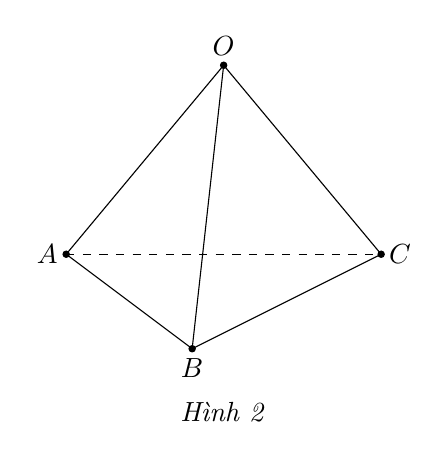
\begin{tikzpicture}[xscale=0.8,yscale=0.8]
				\path
				(0,0) coordinate (A)
				(2,-1.5) coordinate (B)
				(5,0) coordinate (C)
				(2.5,3) coordinate (O)
				;
				\draw[dashed] (A)--(C)
				;
				\draw (A)--(B) (A)--(O) (C)--(B) (B)--(O) (C)--(O)
				;
				\foreach \x/\g in {O/90, A/180, B/-90, C/0} \path (\x) circle (.05) +(\g:.3) node {$\x$}
				;
				\draw (2.5,-2.5) node{\textit{Hình 2}}
				;
				\foreach \x/\g in {O/90, A/90, B/90, C/90} \draw[fill=black] (\x) circle (.05) +(\g:.3) node {}
				;
		\end{tikzpicture}}
	}
\end{vd}
\dongcham{5}

\begin{vd}%[2H3H3-1][Mức độ 2]
	Trong không gian $Oxyz$, cho hai mặt phẳng $(P)\colon 2x+y-z-1=0$ và $(Q)\colon x-2y+z-5=0$. Gọi $\Delta$ là giao tuyến của $(P)$ và $(Q)$. Tìm một điểm thuộc $\Delta$ và một vectơ chỉ phương của $\Delta$.
	\loigiai{
		Mặt phẳng $(P)$ và $(Q)$ có VTPT lần lượt là $\overrightarrow{n}_P=(2;1;-1)$ và $\overrightarrow{n}_Q=(1;-2;1)$.\\
		Vậy vectơ chỉ phương của đường thẳng $d$ là giao tuyến của $(P)$ và $(Q)$ là
		$\overrightarrow{u}=\left[\overrightarrow{n}_P,\overrightarrow{n}_Q\right]=(1;3;5)$.}
\end{vd}
\dongcham{5}
\boxmini{BÀI TẬP TRẮC NGHIỆM}
\setcounter{ex}{0}

\begin{ex}
	Cho đường thẳng $d\colon \heva{&x = 1 + 2t\\&y = - t\\&z = 4 + 5t}$. Đường thẳng $d$ có một vectơ chỉ phương là
	\choice
	{\True $\overrightarrow{u_2} = \left(2;-1;5\right)$}
	{$\overrightarrow{u_4} = \left(1;-1;4\right)$}
	{$\overrightarrow{u_3} = \left(1;-1;5\right)$}
	{$\overrightarrow{u_1} = \left(1;0;4\right)$}
	\loigiai{
		Đường thẳng $d$ có một vectơ chỉ phương là $\overrightarrow{u} = \left(2;-1;5\right)$.}
\end{ex}

\begin{ex}
	Cho đường thẳng $d\colon \dfrac{x-2}{-1}=\dfrac{y-1}{2}=\dfrac{z}{1}$. Đường thẳng $d$ có một vectơ chỉ phương là
	\choice
	{\True $\vec{u}=(-1;2;1)$}
	{ $\vec{u}=(2;1;0)$}
	{ $\vec{u}=(-1;2;0)$}
	{ $\vec{u}=(2;1;1)$}
	\loigiai{
		\textbf{Cần nhớ}: Đường thẳng $d\colon \dfrac{x-x_0}{a} =\dfrac{y-y_0}{b}= \dfrac{z-z_0}{c}$ có một VTCP là $\vec{u}=(a;b;c)$ và đi qua điểm $M(x_0;y_0;z_0)$.\\
		Đường thẳng $d\colon \dfrac{x-2}{-1}=\dfrac{y-1}{2}=\dfrac{z}{1}$ có một vectơ chỉ phương là $\vec{u}=(-1;2;1)$.
	}
\end{ex}

\begin{ex}
	Cho đường thẳng $d: \dfrac{x-1}{2}=\dfrac{y+1}{3}=\dfrac{z}{2}$. Điểm nào trong các điểm dưới đây nằm trên đường thẳng $d$?
	\choice
	{$P(5;2;5)$}
	{$Q(1;0;0)$}
	{\True $M(3;2;2)$}
	{$N(1;-1;2)$}
	\loigiai{
	}
\end{ex}

\begin{ex}
	Cho đường thẳng $d: \begin{cases}
		x=1+2t \\
		y=2+3t \\
		z=5-t
	\end{cases}(t\in \mathbb{R})$. Đường thẳng $d$ \textbf{không} đi qua điểm nào sau đây?
	\choice{$M(1;2;5)$}
	{\True $N(2;3;-1)$}
	{$P(3;5;4)$}
	{$Q(-1;-1;6)$} 
	\loigiai{
	}
\end{ex}

\begin{ex}%[Phát triển đề minh họa, 2021]%[Đoàn Minh Tân]%[2H3Y3-1]%
	Cho hai điểm $A(2;-1;4)$ và $B(-1;3;2)$. Đường thẳng $AB$ có một vectơ chỉ phương là
	\choice
	{$\overrightarrow{u}_1=(1;2;2)$}
	{$\overrightarrow{u}_3=(1;2;6)$}
	{\True $\overrightarrow{u}_2=(3;-4;2)$}
	{$\overrightarrow{u}_4=(1;-4;2)$}
	\loigiai{
		Đường thẳng $AB$ nhận $\overrightarrow{AB}=(-3;4;-2)$ làm một vectơ chỉ phương.\\
		Do đó $\overrightarrow{u}_2=(3;-4;2)=-\overrightarrow{AB}$ cũng là một vectơ chỉ phương của $AB$.
	}
\end{ex}

\begin{ex}%[Paul Hieu Nguyen]%[2H3B3-1]%Câu 35.10
	Cho tam giác $ABC$ với $A(1;0;-2)$, $B(2;-3;-4)$, $C(3;0;-3)$. Gọi $G$ là trọng tâm tam giác $ABC$. vectơ nào sau đây là một vectơ chỉ phương của đường thẳng $OG$?
	\choice
	{\True $(-2;1;3)$}
	{$(3;-2;1)$}
	{$(2;1;3)$}
	{$(-1;-3;2)$}
	\loigiai{
		$G$ là trọng tâm tam giác $ABC \Rightarrow G(2;-1;-3)\Rightarrow \overrightarrow{OG}=(2;-1;-3)$.\\
		Đường thẳng $OG$ nhận $\vec{u}=-\overrightarrow{OG}=(-2;1;3)$ làm một vectơ chỉ phương.
	}
\end{ex}

\begin{ex}
	Cho đường thẳng $d$ song song với trục $Oy$. Đường thẳng $d$ có một vectơ chỉ phương là
	\choice
	{$\overrightarrow{u}_4=(2019;0;2019)$}
	{$\overrightarrow{u}_1=(2019;0;0)$}
	{\True $\overrightarrow{u}_2=(0;2019;0)$}
	{$\overrightarrow{u}_3=(0;0;2019)$}
	\loigiai{
		Trục $Oy$ có vectơ chỉ phương $\overrightarrow{j}=(0;1;0)$, mà $d\parallel Oy$ nên $d$ có một vectơ chỉ phương là \[\overrightarrow{u}_2=2019\overrightarrow{j}=(0;2019;0)\]
	}
\end{ex}

\begin{ex}%[2-TT-41-Vted-lan6-2019]%[Trần Nhân Kiệt, dự án tex đề W-T-B]%[2H3Y3-1]%
	Cho đường thẳng $\Delta$ vuông góc với mặt phẳng $(\alpha) \colon x+2z+3=0$. Một vectơ chỉ phương của $\Delta$ là
	\choice
	{$\overrightarrow{v}=(1;2;3)$}
	{\True $\overrightarrow{a}=(1;0;2)$}
	{$\overrightarrow{u}=(2;0;-1)$}
	{$\overrightarrow{b}=(2;-1;0)$}
	\loigiai{
		Ta có $\Delta$ vuông góc với $(\alpha) \Rightarrow \overrightarrow{a}=(1;0;2)$ là một vectơ chỉ phương của $\Delta$.}
\end{ex}

\begin{ex}%[2H3V3-1][Mức độ 3]
	vectơ chỉ phương của đường thẳng vuông góc với mặt phẳng đi qua ba điểm $A(1;2;4)$, $B(-2;3;5)$, $C(-9;7;6)$ có toạ độ là
	\choice
	{$(3;4;-5)$}
	{$(3;-4;5)$}
	{$(-3;4;-5)$}
	{\True $(3;4;5)$}
	\loigiai{
		Gọi $(P)$ là mặt phẳng đi qua ba điểm $A$, $B$, $C$. \\
		Gọi $\overrightarrow{a}$ là vectơ chỉ phương của đường thẳng $d$ là đường thẳng vuông góc với $(P)$.\\
		Ta có $\overrightarrow{AB}=(-3;1;1),\overrightarrow{AC}=(-10;5;2)$.\\
		Vì $d$ vuông góc với $(P)$ nên $d$ có vectơ chỉ phương là
		$\overrightarrow{a}=\left[\overrightarrow{AB},\overrightarrow{AC}\right]=(-3;-4;-5)=-1(3;4;5)$.}
\end{ex}

\begin{ex}%[2H3B3-1]%
	Cho hai mặt phẳng $(P): 3x-2y+2z-5=0$, $(Q): 4x+5y-z+1=0$. Các điểm $A, B$ phân biệt thuộc giao tuyến của hai mặt phẳng $(P)$ và $(Q)$. Khi đó $\overrightarrow{AB}$ cùng phương với vectơ nào sau đây?
	\choice
	{\True $\overrightarrow{u}=(8;-11;-23)$}
	{$\overrightarrow{k}=(4;5;-1)$}
	{$\overrightarrow{w}=(3;-2;2)$}
	{$\overrightarrow{v}=(-8;11;-23)$}
	\loigiai{
		Ta có $\overrightarrow{n}=(3;-2;2)$ và $\overrightarrow{n'}=(4;5;-1)$ lần lượt là các vectơ pháp tuyến của các mặt phẳng $(P), (Q)$. Do đó $\left[\overrightarrow{n}, \overrightarrow{n'}\right]=(-8;11;23)$ là một vectơ chỉ phương của giao tuyến của $(P)$ và $(Q)$.\\
		Từ đó suy ra $\overrightarrow{AB}$ cùng phương với vectơ $\overrightarrow{u}=(8;-11;-23)$.
	}
\end{ex}

\begin{dang}{Viết phương trình đường thẳng $d$ khi biết vài yếu tố liên quan}
	\begin{itemize}
		\item [\iconCH] \indamm{Phương pháp chung:} Ta cần xác định vectơ chỉ phương $\vec{u}$  và một điểm $M$ thuộc đường thẳng.
		\item [\iconCH] \indamm{Một số kiểu xác định vectơ $\vec{u}$ thường gặp:} 
		\begin{listEX}[1]
			\item [\ding{172}] $d$ qua hai điểm $A$, $B$ thì $\vec{u}=\vec{AB}=(x_B-x_A;y_B-y_A;z_B-z_A)$.
			\item [\ding{173}] $d$ song song với $\Delta$ thì $\vec{u}=\vec{u_{\Delta}}$.
			\item [\ding{174}] $d$ vuông góc với $(P)$ thì $\vec{u}=\vec{n}_{P}$.
			\item [\ding{175}]  $d$ vuông góc với giá của hai vectơ $\vec{a}$ và $\vec{b}$ (không cùng phương) thì $\vec{u}=[\vec{a},\vec{b}]$.
		\end{listEX}
	\end{itemize}
\end{dang}
\boxmini{BÀI TẬP TỰ LUẬN}
\setcounter{vd}{0}

\begin{vd}%[2H5H2-3]%[Dự án tex hóa sách bài tập Toán 12 CTST]%[Lê Thị Thúy Hằng]
	Lập phương trình chính tắc của đường thẳng $d$ trong mỗi trường hợp sau
	\begin{enumerate}
		\item $d$ đi qua điểm $A(4;-2;5)$ và có vectơ chỉ phương $\overrightarrow{a}=(7;3;-9)$.
		\item $d$ đi qua hai điểm $M(0;0;1)$, $N(3;3;6)$.
		\item $d$ có phương trình tham số là $\heva{&x=8+5t\\&y=7+4t\\&z=11+9t.}$
	\end{enumerate}
	\loigiai{
		\begin{enumerate}
			\item Đường thẳng $d$ đi qua điểm $A(4;-2;5)$ và có vectơ chỉ phương $\overrightarrow{a}=(7;3;-9)$ nên $d$ có phương trình chính tắc là
			$\dfrac{x-4}{7}=\dfrac{y+2}{3}=\dfrac{z-5}{-9}$.
			\item Đường thẳng $d$ đi qua hai điểm $M(0;0;1)$, $N(3;3;6)$ nên $d$ có vectơ chỉ phương là $\overrightarrow{MN}=(3;3;5)$.\\
			Suy ra phương trình chính tắc của đường thẳng $d$ là $\dfrac{x}{3}=\dfrac{y}{3}=\dfrac{z-1}{5}$.
			\item Đường thẳng $d$ có phương trình tham số là $\heva{&x=8+5t\\&y=7+4t\\&z=11+9t}$, suy ra $d$ có phương trình chính tắc là $\dfrac{x-8}{5}=\dfrac{y-7}{4}=\dfrac{z-11}{9}$.
		\end{enumerate}
	}
\end{vd}
\dongcham{8}
\begin{vd}
\immini{Trong một khu du lịch, người ta cho du khách trải nghiệm thiên nhiên bằng cách đu theo đường trượt zipline từ vị trí $A$ cao 15 m của tháp 1 này sang vị trí $B$ cao 10 m của tháp 2 trong khung cảnh tuyệt đẹp xung quanh. Với hệ trucuc toạ độ $O x y z$ cho trưóc (đơn vị: mét), toạ độ của $A$ và $B$ lần lượt là $(3 ; 2,5 ; 15)$ và $(21 ; 27,5 ; 10)$.
\begin{enumEX}[a)]{1}
	\item Viết phương trình đường thẳng chứa đường trượt zipline này.
	\item Xác định toạ độ của du khách khi ở độ cao 12 mét.
\end{enumEX}}{
\includegraphics[scale=0.6]{images/2P5-B2-NguyenHuuTinh-H5-23}
}
\end{vd}
\dongcham{5}
\begin{vd}
	Trong không gian $Oxyz$, Lập phương trình tham số và phương trình chính tắc (nếu có) của đường thẳng $d$ trong các trường hợp sau:
	\begin{enumEX}[a)]{1}
		\item $d$ đi qua điểm $M$ và song song với đường thẳng $\Delta \colon \dfrac{x-1}{2}=\dfrac{y+1}{1}=\dfrac{z}{-1}$
		\item $d$ qua điểm $M(3;2;-1)$ và vuông góc với mặt phẳng $(P)\colon x+z-2=0$.
		\item $d$ đi qua điểm $M(1; 2; 1)$, đồng thời vuông góc với cả hai đường thẳng $\Delta_{1}\colon \dfrac{x-2}{1}=\dfrac{y+1}{-1}=\dfrac{z-1}{1}$ và $\Delta_{2}\colon \dfrac{x+1}{1}=\dfrac{y-3}{2}=\dfrac{z-1}{-1}$.
	\end{enumEX}

	\loigiai
	{
		\begin{enumerate}[a)]
			\item Đường thẳng $\Delta$ có vectơ chỉ phương là $\vec{u}=(2;1;-1)$.\\
			Đường thẳng $d$ qua $M(2;1;0)$ và song song với đường thẳng $\Delta$ cũng nhận $\vec{u}=(2;1;-1)$ làm vectơ chỉ phương của nó.\\
			Vậy phương trình đường thẳng cần tìm là
			\[\dfrac{x-2}{2}=\dfrac{y-1}{1}=\dfrac{z}{-1} \Leftrightarrow\dfrac{x-2}{4}=\dfrac{y-1}{2}=\dfrac{z}{-2}.\]
			\item Mặt phẳng $(P)\colon x+z-2=0$ có vectơ pháp tuyến là $\overrightarrow{n}_{(P)}=(1;0;1)$.\\
			Đường thẳng $\Delta$ đi qua $M$ và vuông góc với $(P)$ nhận $\overrightarrow{n}_{(P)}$ làm vectơ chỉ phương có phương trình là
			$$\heva{& x=3+t \\ & y=2\\& z=-1+t.}$$
			\item Đường thẳng $\Delta_{1}$ và $\Delta_{2}$ có vectơ chỉ phương là $\vec{u}_1 =(1;-1;1)$ và $\vec{u}_2=(1;2;-1)$.\\
			Vì $d$ vuông góc với cả hai đường thẳng $\Delta_{1}$ và $\Delta_{2}$ nên $d$ có vectơ chỉ phương là $\vec{u}=\left[\vec{u}_{1}, \vec{u}_{2}\right]=(-1; 2; 3)$.\\
			Vậy phương trình đường thẳng $d$ là $\heva{&x=1-t \\&y=2+2 t\\&z=1+3 t}.$
		\end{enumerate}
		
	}
\end{vd}
\dongcham{18}
\begin{vd}%[2H3V3-2]
	Trong không gian $Oxyz$, cho điểm $A(1;-2;0)$, mặt phẳng $(P)\colon 2x-3y+z+5=0$ và đường thẳng $d\colon \dfrac{x-1}{2}=\dfrac{y}{-1}=\dfrac{z+1}{1}$. Viết phương trình đường thẳng $\Delta$ đi qua $A$, cắt $d$ và song song với mặt phẳng $(P)$.
	\loigiai
	{
		Mặt phẳng $(P)$ có VTPT $\overrightarrow{n}=(2 ;-3 ; 1)$.\\
		Gọi $M$ là giao điểm của $\Delta$ và $d\colon \heva{&x=1+2t\\&y=-t\\&z=-1+t}$ là $M(1+2t ;-t ;-1+t)$.\\
		Đường thẳng $\Delta$ nhận $\overrightarrow{AM}=(2 t ;-t+2 ; t-1)$ làm VTCP.\\
		Đường thẳng $\Delta$ song song với mặt phẳng $(P)$ nên
		$$\overrightarrow{AM} \cdot \overrightarrow{n}=0 \Leftrightarrow 2t \cdot 2+(-t+2)\cdot(-3)+(t-1) \cdot 1=0 \Leftrightarrow t=\dfrac{7}{8}.$$
		Suy ra $\overrightarrow{AM}=\left(\dfrac{7}{4} ; \dfrac{9}{8} ;-\dfrac{1}{8}\right)=\dfrac{1}{8}(14 ; 9 ;-1)$.\\
		Đường thẳng $\Delta$ qua $A$ và nhận $\overrightarrow{AM}=(14 ; 9 ;-1)$ làm VTCP nên phương trình $\Delta\colon \heva{&x=1+14t\\&y=-2+9t\\&z=-t.}$	
	}
\end{vd}
\dongcham{10}

\begin{vd}%[2H3K3-2]%Câu 27%[Đình Phúc ]%
	Trong Không gian với hệ tọa độ $Oxyz$, cho hai đường thẳng $d_1 \colon \dfrac{x-2}{1}=\dfrac{y-1}{-1}=\dfrac{z-2}{-1}$ và $d_2 \colon \heva{&x=t\\&y=3\\&z=-2+t}$. Viết phương trình đường vuông góc chung của hai đường thẳng $d_1, d_2$.
	\loigiai{
		Gọi $d$ là đường thẳng cần tìm.
		Gọi $A=d \cap d_1,B=d \cap d_2$\\
		$\begin{aligned}
			& A \in d_1 \Rightarrow A(2+a;1-a;2-a)\\
			& B \in d_2 \Rightarrow B(b;3;-2+b)\\
			& \overrightarrow{AB}=(-a+b-2;a+2;a+b-4)
		\end{aligned}$\\
		$d_1$ có vectơ chỉ phương $\overrightarrow{a}_1=(1;-1;-1)$,
		$d_2$ có vectơ chỉ phương $\overrightarrow{a}_2=(1;0;1)$\\
		$\heva{&d \perp d_1\\&d \perp d_2} \Leftrightarrow \heva{&\overrightarrow{AB} \perp \overrightarrow{a}_1\\&\overrightarrow{AB} \perp \overrightarrow{a}_2} \Leftrightarrow \heva{&\overrightarrow{AB} \cdot \overrightarrow{a}_1=0\\&\overrightarrow{AB} \cdot \overrightarrow{a}_2=0} \Leftrightarrow \heva{&a=0\\&b=3} \Rightarrow A(2;1;2);B(3;3;1)$\\
		$d$ đi qua điểm $A(2;1;2)$ và có vectơ chỉ phương $\overrightarrow{a}_d=\overrightarrow{AB}=(1;2;-1)$\\
		Vậy phương trình của $d$ là $\heva{&x=2+t\\&y=1+2t\\&z=2-t}$}
\end{vd}
\dongcham{10}
\boxmini{BÀI TẬP TRẮC NGHIỆM}
\setcounter{ex}{0}

\begin{ex}
	Cho đường thẳng $\Delta$ đi qua điểm $M\left(2;0;-1\right)$ và có vectơ chỉ phương $\overrightarrow{a}=\left(4;-6;2\right)$. Phương trình tham số của đường thẳng $\Delta$ là
	\choice
	{$\heva{&x=-2+2t\\& y=-3t\\& z=1+t}$}
	{$\heva{&x=2+2t\\ &y=-3t\\& z=-1+t}$}
	{$\heva{&x=-2+4t\\& y=-6t\\ &z=1+2t}$}
	{\True $\heva{&x=4+2t\\ &y=-3t\\ &z=2+t}$}
	\loigiai{
	}
\end{ex}
\cham{3}

\begin{ex}
	Cho hai điểm $A(2;-1;3), B(3;2;-1)$. Phương trình nào sau đây là phương trình đường thẳng $AB$?
	\choice
	{$\heva{&x=1+2t\\&y=3-t\\&z=-4+3t}$}
	{\True $\heva{&x=2+t\\&y=-1+3t\\&z=3-4t}$}
	{$\heva{&x=2+t\\&y=-1+t\\&z=3-4t}$}
	{$\heva{&x=1+2t\\&y=1-t\\&z=-4+3t}$}
	\loigiai{
	}
\end{ex}
\cham{3}

\begin{ex}
	Cho đường thẳng $\Delta: \dfrac{2x-1}{2}=\dfrac{y}{1}=\dfrac{z+1}{-1}$, điểm $A(2;-3;4)$. Đường thẳng qua $A$ và song song với $\Delta$ có phương trình là
	\choice
	{ $\heva{&x=2+t  \\&	y=-3+t  \\&	z=4-t}$}
	{\True $\heva{&x=2-2t  \\&y=-3-t  \\&	z=4+t}$}
	{$\heva{&x=2+2t  \\&y=-3+t  \\&	z=4+t}$}
	{ $\heva{&x=2+2t  \\&y=1-3t  \\&z=-1+4t}$}
	\loigiai{
	}
\end{ex}
\cham{3}

\begin{ex}
	Viết phương trình đường thẳng đi qua điểm $N(2;-3;-5)$ và vuông góc với mặt phẳng $(P): 2x-3y-z+2=0$.
	\choice
	{\True $\dfrac{x-2}{2}=\dfrac{y+3}{-3}=\dfrac{z+5}{-1}$}
	{$\dfrac{x+2}{2}=\dfrac{y-3}{-3}=\dfrac{z-5}{-1}$}
	{$\dfrac{x+2}{2}=\dfrac{y-3}{-3}=\dfrac{z-1}{-5}$}
	{$\dfrac{x-2}{2}=\dfrac{y+3}{-3}=\dfrac{z+1}{-5}$}
	\loigiai{
	}
\end{ex}
\cham{3}

\begin{ex}
	Cho tam giác $ABC$ có $A(3;2;-4), B(4;1;1)$ và $C(2;6;-3).$ Viết phương trình đường thẳng $d$ đi qua trọng tâm $G$ của tam giác $ABC$ và vuông góc với mặt phẳng $(ABC)$.
	\choice
	{$d:\dfrac{x-3}{3}=\dfrac{y-3}{2}=\dfrac{z+2}{-1}$}
	{$d:\dfrac{x+12}{3}=\dfrac{y+7}{2}=\dfrac{z-3}{-1}$}
	{\True $d:\dfrac{x-3}{7}=\dfrac{y-3}{2}=\dfrac{z+2}{-1}$}
	{$d:\dfrac{x+7}{3}=\dfrac{y+3}{2}=\dfrac{z-2}{-1}$}
	\loigiai{
	}
\end{ex}
\cham{3}

\begin{ex}%[2H3V3-2]
	Cho hai điểm $A(1;-1;1)$ và $B(-1;2;3)$ và đường thẳng $\Delta\colon\dfrac{x+1}{-2}=\dfrac{y-2}{1}=\dfrac{z-3}{3}$. Phương trình đường thẳng đi qua điểm $A$, đồng thời vuông góc với hai đường thẳng $AB$ và $\Delta$ là
	\choice
	{$\dfrac{x+1}{7}=\dfrac{y-1}{-2}=\dfrac{z+1}{4}$}
	{$\dfrac{x+1}{7}=\dfrac{y-1}{2}=\dfrac{z+1}{4}$}
	{$\dfrac{x-7}{1}=\dfrac{y-2}{-1}=\dfrac{z-4}{1}$}
	{\True $\dfrac{x-1}{7}=\dfrac{y+1}{2}=\dfrac{z-1}{4}$}
	\loigiai{
		Ta có: $\overrightarrow{AB}=(-2;3;2)$.\\
		Đường thẳng $\Delta$ có vectơ chỉ phương là $\overrightarrow{u}_{\Delta}=(-2;1;3)\Rightarrow\left[\overrightarrow{AB},\overrightarrow{u}_{\Delta}\right]=(7;2;4)$.\\
		Đường thẳng đi qua điểm $A$, đồng thời vuông góc với hai đường thẳng $AB$ và $\Delta$ có vectơ chỉ phương $\left[\overrightarrow{AB},\overrightarrow{u}_{\Delta}\right]$ có phương trình là $\dfrac{x-1}{7}=\dfrac{y+1}{2}=\dfrac{z-1}{4}$.}
\end{ex}
\cham{4}

\begin{ex}
	Cho điểm $A(1;2;3)$ và đường thẳng $d: \dfrac{x+1}{2}=\dfrac{y}{1}=\dfrac{z-3}{-2}$. Gọi $\Delta$ là đường thẳng đi qua điểm $A$, vuông góc với đường thẳng $d$ và cắt trục hoành. Tìm một vectơ chỉ phương $\overrightarrow{u}$ của đường thẳng $\Delta$.
	\choice
	{$\overrightarrow{u}=(0;2;1)$}
	{$\overrightarrow{u}=(1;0;1)$}
	{$\overrightarrow{u}=(1;-2;0)$}
	{\True $\overrightarrow{u}=(2;2;3)$}
	\loigiai{
	}
\end{ex}
\cham{5}

\begin{ex}
	Cho hai đường thẳng $d_1: \dfrac{x-1}{1}=\dfrac{y+1}{2}=\dfrac{z}{-1}$ và $d_2: \dfrac{x-2}{1}=\dfrac{y}{2}=\dfrac{z+3}{2}$. Viết phương trình đường thẳng $\Delta$ đi qua điểm $A(1;0;2)$, cắt $d_1$ và vuông góc với $d_2$.
	\choice
	{$\dfrac{x-1}{-2}=\dfrac{y}{3}=\dfrac{z-2}{4}$}
	{\True $\dfrac{x-3}{2}=\dfrac{y-3}{3}=\dfrac{z+2}{-4}$}
	{$\dfrac{x-5}{-2}=\dfrac{y-6}{-3}=\dfrac{z-2}{4}$}
	{$\dfrac{x-1}{-2}=\dfrac{y}{3}=\dfrac{z-2}{-4}$}
	\loigiai{
		Gọi $B(1+t;-1+2t;-t) \in d_1$. Do đó $\overrightarrow{AB}=(t;2t-1;-t-2)$.\\
		Xét $\overrightarrow{AB}.\overrightarrow{u}_{d_2}=0 \Longleftrightarrow 1.t +2(2t-1)+2(-t-2)=0\Longleftrightarrow t=2$.\\
		Ta có $\overrightarrow{AB}=(2;3;-4)$ chính là vec-tơ chỉ phương của đường thẳng $\Delta$.\\
		Vậy phương trình đường thẳng $\Delta$ là $\heva{x=1+2t\\y=3t\\z=2-4t}$.\\
		Với $t=1$ thì đường thẳng $\Delta$ đi qua điểm $C(3;3;-2)$.\\
		Vậy phương trình đường thẳng $\Delta$ là $\dfrac{x-3}{2}=\dfrac{y-3}{3}=\dfrac{z+2}{-4}$.
	}
\end{ex}
\cham{5}
\begin{ex}%[Paul Hieu Nguyen]%[2H3K3-2]%Câu 35.16
	Cho đường thẳng $\Delta$ đi qua $M(1;2;2)$, song song với mặt phẳng
	$(P)\colon x-y+z+3=0$ đồng thời cắt đường thẳng $d\colon \dfrac{x-1}{1}=\dfrac{y-2}{1}=\dfrac{z-3}{1}$ có phương trình là
	\def\dotEX{}
	\choice
	{\True $\heva{&x=1-t\\&y=2-t\\&z=2.}$}
	{$\heva{&x=1\\&y=2-t\\&z=2-t.}$}
	{$\heva{&x=1-t\\&y=2+t\\&z=2.}$}
	{$\heva{&x=-1+t\\&y=-1+2t\\&z=2t.}$}
	\loigiai{
		Đường thẳng $d$ có phương trình tham số là $\heva{&x=1+t\\&y=2+t\\&z=3+t.}$\\
		Mặt phẳng $(P)$ có một VTPT là $\vec{n}_P=(1;-1;1)$.\\
		Giả sử $\Delta$ cắt $d$ tại $A$
		$\Rightarrow A(1+t;2+t;3+t)$ và $\overrightarrow{MA}=(t;t;1+t)$.\\
		Vì $\Delta$ song song $(P)$ nên $\overrightarrow{MA}\cdot\vec{n}=0\Leftrightarrow t=-1\Rightarrow \overrightarrow{MA}=(-1;-1;0)$.\\
		Chọn một VTCP của $\Delta$ là $\vec{u}_{\Delta}=\overrightarrow{MA}=(-1;-1;0)$.\\
		Đường thẳng $\Delta$ có phương trình tham số là $\heva{&x=1-t\\&y=2-t\\&z=2.}$
	}
\end{ex}
\begin{ex}%%[THPT Việt Đức_Hà Nội_HK2] %[2H3K3]
	Cho đường thẳng $d: x=y=z$. Viết phương trình đường thẳng $d'$ là hình chiếu vuông góc của $d$ lên mặt phẳng tọa độ $(Oyz)$. 
	\choice
	{$\heva{&x=0\\&	y=t \\&	z=2t}$}
	{$\heva{&x=t\\&y=t \\&z=2t}$}
	{$\heva{&x=0\\&y=2+t \\&z=1+t}$}
	{\True $\heva{&x=0\\&y=t \\&z=t}$}
	\loigiai{
	}
\end{ex}
\cham{5}

\begin{ex}
	Cho đường thẳng $d:\dfrac{x+1}{2}=\dfrac{y}{1}=\dfrac{z-2}{1},$ mặt phẳng $(P):x+y-2z+5=0$ và điểm $A(1;-1;2).$ Viết phương trình đường thẳng $\Delta$ cắt $d$ và $(P)$ lần lượt tại $M$ và $N$ sao cho $A$ là trung điểm của đoạn thẳng $MN$.
	\choice
	{\True $\Delta:\dfrac{x-3}{2}=\dfrac{y-2}{3}=\dfrac{z-4}{2}$}
	{$\Delta:\dfrac{x-1}{6}=\dfrac{y+1}{1}=\dfrac{z-2}{2}$}
	{$\Delta:\dfrac{x+5}{6}=\dfrac{y+2}{1}=\dfrac{z}{2}$}
	{$\Delta:\dfrac{x+1}{2}=\dfrac{y+4}{3}=\dfrac{z-3}{2}$}
	\loigiai{
		Ta loại ngay được $1$ phương án vì điểm A không thuộc đường thẳng này.\\
		Đường thẳng $d$ có phương trình tham số $d:\left\{\begin{aligned}x&=-1+2t\\y&=t\\z&=2+t\end{aligned}\right.$\\
		$M\in d\Rightarrow M(-1+2t;t;2+t), A$ là trung điểm $MN\Rightarrow N(3-2t;-2-t;2-t)$\\
		$N\in (P)\Rightarrow 3-2t-2-t-2(2-t)+5=0\Leftrightarrow t=2\Rightarrow N(-1;-4;0)\Rightarrow \overrightarrow{NA}=(2;3;2).\Rightarrow $ Loại được hai phương án không thỏa mãn điều kiện này.\\
		Còn duy nhất $1$ phương án cần chọn.
	}
\end{ex}
\cham{5}
\begin{ex}%[Đề thi HK2, môn Toán THPT Yên Lạc, Vĩnh phúc]%[Nguyễn Quang Dũng, dự án 12-EX-6-2020]%[2H3K3-2]%
	Trong không gian $Oxyz$, đường vuông góc chung của hai đường thẳng chéo nhau $d_1\colon \dfrac{x-2}{2}=\dfrac{y-3}{3}=\dfrac{z+4}{-5}$ và $d_2\colon \dfrac{x+1}{3}=\dfrac{y-4}{-2}=\dfrac{z-4}{-1}$ có phương trình là
	\choice
	{$\dfrac{x-2}{2}=\dfrac{y+2}{2}$}
	{$\dfrac{x-2}{2}=\dfrac{y-2}{3}=\dfrac{z-3}{4}$}
	{\True $\dfrac{x}{1}=\dfrac{y}{1}=\dfrac{z-1}{1}$}
	{$\dfrac{x}{2}=\dfrac{y-2}{3}=\dfrac{z-3}{-1}$}
	\loigiai{
		Giả sử $M\in d_1$, $N\in d_2$ và $MN$ là đoạn vuông góc chung.\\
		Ta có $M(2+2t;3+3t;-4-5t)\,\,N(-1+3s;4-2s;4-s)$, $\overrightarrow{MN}=(3s-2t-3;-2s-3t+1;-s+5t+8)$.\\
		vectơ chỉ phương của $d_1$, $d_2$ lần lượt là $\overrightarrow{u}_1=(2;3;-5)$, $\overrightarrow{u}_2=(3;-2;-1)$. \\
		Ta có $MN$ là đoạn vuông góc chung của $d_1$ và $d_2$ khi và chỉ khi
		\[\heva{&\overrightarrow{MN}\cdot\overrightarrow{u}_1=0\\&\overrightarrow{MN}\cdot\overrightarrow{u}_2=0}\Leftrightarrow\heva{&5s-38t-43=0\\&14s-5t-19=0}\Leftrightarrow\heva{&t=-1\\&s=1.}\]
		Suy ra $M(0;0;1)$, $\overrightarrow{MN}=(2;2;2)$. Ta có phương trình của đường vuông góc chung $MN$ là
		\[\dfrac{x}{1}=\dfrac{y}{1}=\dfrac{z-1}{1}.\]
	}
\end{ex}
\begin{dang}{Vị trí tương đối của hai đường thẳng}
	Cho $d$ qua điểm $M$ và có vectơ chỉ phương $\vec{u}$; $d'$ qua điểm $N$ và có vectơ chỉ phương $\vec{v}$.
	\begin{listEX}[1]
		\item [\ding{172}] Nếu $\vec{u}$ cùng phương $\vec{v}$ ($\vec{u}=k\vec{v}$) và $M \notin d'$ thì $d \parallel d'$.
		\item [\ding{173}] Nếu $\vec{u}$ cùng phương $\vec{v}$ ($\vec{u}=k\vec{v}$) và $M \in d'$ thì $d$ trùng với $d'$.
		\item [\ding{174}] Nếu $\left[\vec{u},\vec{v}\right] \cdot \vec{MN} \ne 0$ thì $d$ và $d'$ chéo nhau.
		\item [\ding{175}] Nếu $\left[\vec{u},\vec{v}\right] \cdot \vec{MN} = 0$ thì $d$ và $d'$ cắt nhau.
		\item [\ding{176}] Nếu $\vec{u} \cdot \vec{v} =0$ thì $d$ và $d'$ vuông góc nhau.
	\end{listEX}
\end{dang}
\boxmini{BÀI TẬP TỰ LUẬN}
\begin{vd}%[2H5V2-4]
	\immini{
		Trên phần mềm mô phỏng 3D một máy khoan trong không gian $Oxyz$, cho biết phương trình trục $a$ của mũi khoan và một đường rãnh $b$ trên vật cần khoan (tham khảo hình vẽ bên) lần lượt là $$a\colon\heva{& x=1\\&y=2\\&z=3t }\text{ và }b\colon\heva{& x=1+4t'\\&y=2+2t'\\&z=6. }$$
		\begin{enumerate}
			\item Chứng minh $a$, $b$ vuông góc và cắt nhau.
			\item Tìm giao điểm của $a$ và $b$.
		\end{enumerate}
	}{
		\includegraphics[scale=0.3]{images/12-SGK-CTST-5-2-13}
	}
	\loigiai
	{
		\begin{enumerate}
			\item $a$ có vectơ chỉ phương $\overrightarrow{m}=(0;0;3)$ và $b$ có vectơ chỉ phương $\overrightarrow{n}=(4;2;0)$.\\
			Ta có $\overrightarrow{m}\cdot\overrightarrow{n}=0\cdot 4+0\cdot 2+3\cdot 0=0$.\\
			Do đó $\overrightarrow{m}\perp\overrightarrow{n}$ hay $a\perp b$.
			\item Gọi $M$ là giao điểm của $a$ và $b$, ta có $\heva{& M\in a\\&M\in b }\Rightarrow\heva{& M(1;2;3t)\\&M(1+4t';2+2t';6)}$. Khi đó ta có $$\heva{& 1=1+4t'\\&2=2+2t'\\&3t=6 }\Rightarrow\heva{& t=2\\&t'=0 }\Rightarrow M(1;2;6).$$
			Vậy giao điểm của $a$ và $b$ là $M(1;2;6)$.
		\end{enumerate}
	}
\end{vd}
\dongcham{6}

\setcounter{vd}{0}
\begin{vd}
	Trong khôn gian $Oxyz$, xét vị trí tương đối giữa hai đường thẳng $d$ và $d'$ trong mỗi trường hợp sau. Nếu chúng cắt nhau, hãy xác định tọa độ giao điểm.
	\begin{enumerate}
		\item $d \colon \heva{&x=2+3t\\&y=3+2t\\&z=4+2t}$ và $d' \colon \heva{&x=8+9t'\\&y=7+6t'\\&z=8+6t';}$
		\item $d \colon \dfrac{x}{4}=\dfrac{y-3}{3}=\dfrac{z-1}{2}$ và $d' \colon \dfrac{x-5}{8}=\dfrac{y-5}{6}=\dfrac{z-3}{4}$;
		\item $d \colon \heva{&x=2\\&y=3+2t\\&z=1-t}$ và $d' \colon \dfrac{x-4}{3}=\dfrac{y-1}{4}=\dfrac{z-5}{5}$;
		\item $d \colon \dfrac{x-2}{3}=\dfrac{y-3}{4}=\dfrac{z-2}{3}$ và $d' \colon \heva{&x=5\\&y=7+2t\\&z=5-t.}$
	\end{enumerate}
	\loigiai{
		\begin{enumerate}
			\item Đường thẳng $d$ đi qua điểm $M(2;3;4)$ và nhận $\overrightarrow{a}=(3;2;2)$ làm vectơ chỉ phương.\\
			Đường thẳng $d'$ đi qua điểm $M'(8;7;8)$ và nhận $\overrightarrow{a'}=(9;6;6)$ làm vectơ chỉ phương.\\
			Ta có $\overrightarrow{MM'}=(6;4;4)$, $\overrightarrow{a'} = 3 \overrightarrow{a} = \dfrac{3}{2} \overrightarrow{MM'}$, suy ra ba vectơ $\overrightarrow{a}$, $\overrightarrow{a'}$, $\overrightarrow{MM'}$ cùng phương. Do đó, $d \equiv d'$.
			\item Đường thẳng $d$ đi qua điểm $M(0;3;1)$ và nhận $\overrightarrow{a}=(4;3;2)$ làm vectơ chỉ phương.\\
			Đường thẳng $d'$ đi qua điểm $M'(5;5;3)$ và nhận $\overrightarrow{a'}=(8;6;4)$ làm vectơ chỉ phương.\\
			Ta có $\overrightarrow{MM'}=(5;2;2)$, $\overrightarrow{a'} = 2\overrightarrow{a}$, suy ra $\overrightarrow{a}$, $\overrightarrow{a'}$ cùng phương. Mặt khác, $\dfrac{4}{5} \ne \dfrac{3}{2}$, suy ra $\overrightarrow{a}$, $\overrightarrow{MM'}$ không cùng phương. Do đó $d \parallel d'$.
			\item Đường thẳng $d$ đi qua điểm $M(2;3;1)$ và nhận $\overrightarrow{a}=(0;2;-1)$ làm vectơ chỉ phương.\\
			Đường thẳng $d'$ đi qua điểm $M'(4;1;5)$ và nhận $\overrightarrow{a'}=(3;4;5)$ làm vectơ chỉ phương.\\
			Ta có $\overrightarrow{MM'}=(2;-2;4)$, $\left[ \overrightarrow{a}, \overrightarrow{a'} \right] = (14;-3;-6) \ne \overrightarrow{0}$, $\left[ \overrightarrow{a}, \overrightarrow{a'} \right] \cdot \overrightarrow{MM'} =10 \ne 0$, suy ra $d$ và $d'$ chéo nhau.
			item Đường thẳng $d$ đi qua điểm $M(2;3;2)$ và nhận $\overrightarrow{a}=(3;4;3)$ làm vectơ chỉ phương.\\
			Đường thẳng $d'$ đi qua điểm $M'(5;7;5)$ và nhận $\overrightarrow{a'}=(0;2;-1)$ làm vectơ chỉ phương.\\
			Ta có $\overrightarrow{MM'}=(3;4;3)$, $\left[ \overrightarrow{a}, \overrightarrow{a'} \right] = (-10;3;6) \ne \overrightarrow{0}$, $\left[ \overrightarrow{a}, \overrightarrow{a'} \right] \cdot \overrightarrow{MM'} =0 \ne 0$, suy ra $d$ và $d'$ cắt nhau.
		\end{enumerate}
	}
\end{vd}
\dongcham{29}
\boxmini{BÀI TẬP TRẮC NGHIỆM}
\setcounter{ex}{0}

\begin{ex} %[2H3B3-6]%Câu 9:
	Cho hai đường thẳng $d\colon \heva{&x=1+t \\& y=2 t \\& z=2-t} \text{ và } d'\colon \heva{&x=2+2t' \\& y=3+4t' \\& z=5-2t'.}$ Mệnh đề nào sau đây đúng?
	\choice
	{$d$ và $d'$ chéo nhau}
	{$d$ trùng $d'$}
	{\True $d$ song song $d'$}
	{$d$ cắt $d'$}
	\loigiai{
		$d$ đi qua $A=(1;0;2)$, có vectơ chỉ phương $\vec{a}=(1;2;-1).$\\
		$d'$ đi qua $B=(2;3;5)$, có vectơ chỉ phương $\vec{a'}=(2;4;-2).$\\
		Ta có $\vec{a}$ cùng phương $\vec{a'}$ nên loại B. D.\\
		$A \notin d'$ nên $d$ song song $d'$.
	}
\end{ex}
\cham{5}

\begin{ex} %[2H3B3-6]%Câu 11:
	Cho hai đường thẳng $d_1 \colon \dfrac{x-1}{1}=\dfrac{y+3}{-2}=\dfrac{z+3}{-3}$ và $d_2\colon \heva{&x=3t \\& y=-1+2t \\& z=0}$. Mệnh đề nào đưới đây đúng?
	\choice
	{\True $d_1$ cắt và không vuông góc với $d_2$}
	{$d_1$ cắt và vuông góc với $d_2$}
	{$d_1$ song song $d_2$}
	{$d_1$ chéo $d_2$}
	\loigiai{
		$d_1$ đi qua $A=(1;-3;-3)$, có vectơ chỉ phương $\vec{a}_1=(1;-2;-3).$\\
		$d_2$ đi qua $B=(0;-1;0)$, có vectơ chỉ phương $\vec{a}_2=(3;2;0).$\\
		Ta có $\vec{a}_1$ không cùng phương $\vec{a}_2$.\\
		$\vec{a}_1 \cdot \vec{a}_2 \ne 0 $.\\
		$[\vec{a}_1 , \vec{a}_2]\cdot \vec{AB} = 0$ nên $d_1$ cắt và không vuông góc với $d_2$.
	}
\end{ex}
\cham{5}
\begin{ex}
	Cho hai đường thẳng $d_1\colon\heva{&x=1-2t\\&y=1+t\\&z=1-t}$ và $d_2\colon\dfrac{x+1}{2}=\dfrac{y-2}{-1}=\dfrac{z}{1}$. Chọn khẳng định đúng.
	\choice
	{$d_1\parallel d_2$}
	{\True $d_1\equiv d_2$}
	{$d_1$, $d_2$ chéo nhau}
	{$d_1$, $d_2$ cắt nhau}
	\loigiai{
		Ta có $d_1$, $d_2$ có vectơ chỉ phương lần lượt là $\overrightarrow{u}_1=(-2;1;-1)$, $\overrightarrow{u}_2=(2;-1;1)$. \\
		Và $A(1;1;1)\in d_1$, $B(-1;2;0)\in d_2\Rightarrow \overrightarrow{AB}=(-2;1;-1)$.\\
		Khi đó $\overrightarrow{u}_1$, $\overrightarrow{u}_2$, $\overrightarrow{AB}$ cùng phương nên $d_1\equiv d_2$.
	}
\end{ex}

\begin{ex}
	Vị trí tương đối của hai đường thẳng $\Delta _1 \colon \dfrac{x-1}{3}=y=\dfrac{z+1}{2}$ và $\Delta _2 \colon \dfrac{x}{2}=\dfrac{y-1}{-1}=\dfrac{z}{1}$,
	\choice
	{Trùng nhau }
	{\True Chéo nhau}
	{Song song}
	{Cắt nhau}
	\loigiai{
		Đường thẳng	$\Delta _1$ đi qua điểm $M_1\left(1;0;-1\right)$ và có vectơ chỉ phương $\overrightarrow{u_1}=\left(3;1;2\right)$.\\
		Đường thẳng $\Delta _2$ đi qua điểm $M_2\left(0;1;0\right)$ và có vectơ chỉ phương $\overrightarrow{u_2}=\left(2;-1;1\right)$.\\
		Ta có $\heva{& \overrightarrow{u_1}\wedge \overrightarrow{u_2}=\left(3;1;-5\right)\\& \overrightarrow{M_1M_2}=(-1;1;1)} \Rightarrow \left(\overrightarrow{u_1}\wedge \overrightarrow{u_2}\right)\cdot \overrightarrow{M_1M_2}=-3+1-5=-7\ne 0$.\\
		Do đó $\Delta _1$ và $\Delta _2$ chéo nhau.
	}
\end{ex}
\begin{ex}
	Cho hai đường thẳng $d_1:\dfrac{x+1}{2}=\dfrac{y-1}{-m}=\dfrac{z-2}{-3}$ và $d_2: \dfrac{x-3}{1}=\dfrac{y}{1}=\dfrac{z-1}{1}$. Tìm tất cả các giá trị thực của $m$ để $d_1$ vuông góc $d_2$.
	\choice
	{$m=5$}
	{$m=1$}
	{$m=-5$}
	{\True$m=-1$}
	\loigiai{
	}
\end{ex}
\cham{5}

\begin{ex}%[Kiểm tra, Sở GD và ĐT - Khánh Hòa, 2019]%[Thanh Ta, 12EX6]%[2H3B3-6]%
	Cho hai đường thẳng $\Delta_1\colon \dfrac{x-1}{2}=\dfrac{y-2}{3}=\dfrac{z-3}{4}$ và $\Delta_2\colon \dfrac{x-4}{1}=\dfrac{y-3}{-2}=\dfrac{z-5}{-2}$. Tọa độ giao điểm $M$ của hai đường thẳng đã cho là
	\choice
	{$M(5;1;3)$}
	{$M(0;-1;-1)$}
	{\True $M(3;5;7)$}
	{$M(2;3;7)$}
	\loigiai{
		Phương trình tham số của đường thẳng $\Delta_1$ là $\Delta_1\colon\heva{& x=1+2t \\ & y=2+3t\\ &z=3+4t}$, thay vào phương trình $\Delta_2$ ta được
		$$\dfrac{2t-3}{1}=\dfrac{3t-1}{-2}=\dfrac{4t-2}{-2}\Rightarrow t=1.$$
		Vậy giao điểm của $\Delta_1$ và $\Delta_2$ là $M(3;5;7)$.
	}
\end{ex}
\begin{ex}%[Thi Thử Lần 2, THPT Lương Thế Vinh - Hà Nội, 2019]%[Dương BùiĐức, dự án 12EX6]%[2H3B3-6]%
	Cho hai đường thẳng $d_1\colon\heva{
		&x=1+t\\ &y=2-t\\ &z=3+2t
	}$ và $d_2\colon\dfrac{x-1}{2}=\dfrac{y-m}{1}=\dfrac{z+2}{-1}$ (với $m$ là tham số). Tìm $m$ để hai đường thẳng $d_1,\ d_2$ cắt nhau.
	\choice
	{\True $m=5$}
	{$m=7$}
	{$m=9$}
	{$m=4$}
	\loigiai{
		Ta có $ M_{1}(1;2;3)\in d_{1} $ và vectơ chỉ phương của $ d_{1} $ là $ \overrightarrow{u}_{1}=(1;-1;2) $, $ M_{2}(1;m;-2)\in d_{2} $ và vectơ chỉ phương của $ d_{2} $ là $ \overrightarrow{u}_{2}=(2;1;-2) $. Suy ra $ \overrightarrow{M_{1}M_{2}}=(0;m-2;-5) $ và $ [\overrightarrow{u}_{1},\overrightarrow{u}_{2}]=(0;6;3) $.\\
		Để $ d_{1} $ cắt $ d_{2} $ thì $ [\overrightarrow{u}_{1},\overrightarrow{u}_{2}]\cdot \overrightarrow{M_{1}M_{2}}=0\Leftrightarrow 6(m-2)-15=0\Leftrightarrow m=5 $.
	}
\end{ex}
\cham{6}
\begin{ex}
	Cho hai đường thẳng $d: \left \lbrace \begin{aligned} &x=1+mt\\ &y=t  \\&z=-1+2t   \end{aligned} \right. (t \in \mathbb{R})$ và $d': \left \lbrace \begin{aligned} &x=1-t'\\ &y=2+2t'\\&z=3-t'   \end{aligned} \right. (t' \in \mathbb{R})$. Giá trị của $m$ để hai đường thẳng $d$ và $d'$ cắt nhau là
	\choice
	{\True $m=0$}
	{$m=1$}
	{$m=-1$}
	{$m=2$}
	\loigiai{
		Đường thẳng $d$ đi qua $A(1;0;-1)$, có vectơ chỉ phương $\overrightarrow{u_1}=(m;1;2)$.\\
		Đường thẳng $d'$ đi qua $B(1;2;3)$, có vectơ chỉ phương $\overrightarrow{u_2}=(-1;2;-1)$.\\
		Ta có $[\overrightarrow{u_1}, \overrightarrow{u_2}]=(-5;m-2;2m+1)$ và $\overrightarrow{AB}=(0;2;4)$.\\
		Hai đường thẳng $d$ và $d'$ cắt nhau $\Leftrightarrow [\overrightarrow{u_1}, \overrightarrow{u_2}]\cdot AB=0\Leftrightarrow m=0$.
	}
\end{ex}
\begin{dang}{Vị trí tương đối của đường thẳng và mặt phẳng}
	Xét đường thẳng $d \colon \heva{&x=x_0+u_1t\\&y=y_0+u_2t\\&z=z_0+u_3t}$ và mặt phẳng $(P) \colon Ax + By + Cz + D =0$.
	\begin{itemize}
		\item [\iconMT] \indam{Phương pháp:} Xét $d \cap (P) \Rightarrow A(x_0+u_1t)+B(y_0+u_2t)+C(z_0+u_3t)+D=0 \quad (*)$
		\begin{boxdn}
			\begin{itemize}
				\item [$\bullet$] Nếu (*) có đúng 1 nghiệm $t$ thì $d$ cắt $(P)$;
				\item [$\bullet$] Nếu (*) vô nghiệm  thì $d$ song song $(P)$;
				\item [$\bullet$] Nếu (*) nghiệm đúng với mọi $t$ thì $d$ nằm trong $(P)$.
			\end{itemize}
		\end{boxdn}
		\item [\iconMT] \indam{Đặc biệt:} Với $\vec{u}$ là vectơ chỉ phương của $d$ và $\vec{n}$ là vectơ pháp tuyến của $(P)$ thì
		$$d \perp (P) \Leftrightarrow \vec{u} \text{ cùng phương với } \vec{n} \text{ hay } \vec{u}=k \cdot\vec{n}$$
	\end{itemize}
\end{dang}
\boxmini{BÀI TẬP TỰ LUẬN}
\setcounter{vd}{0}

\begin{vd}
	Xét vị trí tương đối giữa đường thẳng và mặt phẳng được chỉ ra ở các câu sau:
	\begin{enumEX}[a)]{1}
		\item $(\alpha) \colon y+2z=0$ và $d \colon \heva{& x=2-t \\ & y=4+2t \\ &z=1} $.
		\item $(P)\colon3x-3y+2z-5=0$ và $d\colon\heva{&x=-1+2t\\&y=3+4t\\&z=3t}~(t\in\mathbb{R})$.
		\item $(P)\colon 3x-3y+2z+1=0$ và $d\colon \dfrac{x+1}{1}=\dfrac{y}{-1}=\dfrac{z-1}{-3}$.
	\end{enumEX}
	\loigiai{
			\begin{enumEX}[a)]{1}
			\item Gọi $M(2-t;4+2t;1) \in d$, thay tọa độ $M$ vào phương trình của $(\alpha)$ ta được $4+2t+2=0 \Leftrightarrow t=-3$. Từ đó tìm được $M(5;-2;1)$. Suy ra $d$ cắt $(\alpha)$.
			\item Xét phương trình $3(-1+2t)-3(3+4t)+2\cdot3t-5=0\Leftrightarrow 0\cdot t-17=0$ (vô nghiệm).\\
			Vậy $d\parallel (P)$.
			\item Viết lại đường thẳng $d$ ở dạng tham số $\heva{&x=-1+t\\&y=-t\\&z=1-3t}$.\\
			Xét phương trình $3\cdot (-1+t)-3\cdot (-t)+2\cdot (1-3t)+1=0 \Leftrightarrow 0=0$. Kết luận phương trình có vô số nghiệm $\Rightarrow d \subset (P)$.
		\end{enumEX}
	}
\end{vd}
\dongcham{15}

\begin{vd}
	Tìm điều kiện của tham số $m$ để
	\begin{enumEX}[a)]{1}
		\item $ \Delta:\dfrac{x-10}{5}=\dfrac{y-2}{1}=\dfrac{z+2}{1}$ vuông góc với $(P):10x+2y+mz+11=0$.
		\item $d\colon \dfrac{x-1}{2}=\dfrac{y+1}{3}=\dfrac{z-1}{-1}$ song song với $(\alpha)\colon -x+m^2y+mz+1=0$.
	\end{enumEX}
	\loigiai{
	\begin{enumEX}[a)]{1}
		\item Đường thẳng $ \Delta $ có VTCP ${\overrightarrow{u}}_{\Delta}=(5;1;1)$. \\
		Mặt phẳng $(P)$ có VTPT ${\overrightarrow{n}}_P=(10;2;m)$. \\
		Để $ \Delta \perp (P) \Leftrightarrow {\overrightarrow{u}}_{\Delta}\parallel {\overrightarrow{n}}_P \Leftrightarrow \dfrac{10}{5}=\dfrac{2}{1}=\dfrac{m}{1} \Leftrightarrow m=2$.
		\item Đường thẳng $d$ có phương trình tham số $\heva{&x=1+2t\\&y=-1+3t\\&z=1-t.}$\\
		Xét phương trình $-(1+2t)+m^2(-1+3t)+m(1-t)+1=0\Leftrightarrow \left(3m^2-m-2\right)t-m^2+m=0.\quad (1)$\\
		Ta có $d\parallel (\alpha)$ khi và chỉ khi $(1)$ vô nghiệm $\Leftrightarrow \heva{&3m^2-m-2=0\\&-m^2+m\neq 0}\Leftrightarrow m=-\dfrac{2}{3}$.
	\end{enumEX}}
\end{vd}
\dongcham{12}
\boxmini{BÀI TẬP TRẮC NGHIỆM}
\setcounter{ex}{0}
\begin{ex}
	Cho đường thẳng $d:\,\displaystyle\frac{x-1}{2}=\frac{y}{-2}=\dfrac{z-1}{1}$. Tìm tọa độ giao điểm $ M $ của đường thẳng $ d $ với mặt phẳng ($ Oxy $).
	\choice
	{\True$M(-1;2;0) $}
	{$ M(1;0;0)$}
	{$ M(2;-1;0)$}
	{$ M(3;-2;0)$}
	\loigiai{
	}
\end{ex}
\cham{3}

\begin{ex}
	Cho đường thẳng $d: \dfrac{x-1}{-1}=\dfrac{y+3}{2}=\dfrac{z-3}{1}$ và mặt phẳng $(P): 2x+y-2z+9=0$. Tìm toạ độ giao điểm của $d$ và $(P)$.
	\choice
	{$(2; 1; 1)$}
	{\True $(0;-1;4)$}
	{$(1; -3; 3)$}
	{$(2; -5; 1)$} 
	\loigiai{
	}
\end{ex}
\cham{4}
\begin{ex}
	Cho mặt phẳng $(\alpha)\colon x+2y+3z-6=0$ và đường thẳng $\Delta\colon\dfrac{x+1}{-1}=\dfrac{y+1}{-1}=\dfrac{z-3}{1}$. Mệnh đề nào sau đây đúng?
	\choice
	{$\Delta$ cắt và không vuông góc với $(\alpha)$}
	{$\Delta\parallel (\alpha)$}
	{\True $\Delta\subset (\alpha)$}
	{$\Delta \perp (\alpha)$}
	\loigiai{
		Mặt phẳng $(\alpha)$ có vectơ pháp tuyến $\overrightarrow{n}=(1;2;3)$.\\
		Đường thẳng $\Delta$ đi qua $M(-1;-1;3)$ và có vectơ chỉ phương $\overrightarrow{u}=(-1;-1;1)$.\\
		Ta có $\overrightarrow{n}\cdot\overrightarrow{u}=1\cdot (-1)+2\cdot (-1)+3\cdot 1=0$ và $M\in (\alpha)$.\\
		Vậy $\Delta\subset (\alpha)$.
	}
\end{ex}

\begin{ex}
	Cho đường thẳng $d:\dfrac{x-1}{1}=\dfrac{y-1}{4}=\dfrac{z-m}{-1}$ và mặt phẳng $(P): 2x+my-(m^2+1)z+m-2m^2=0$. Có bao nhiêu giá trị của $m$ để đường thẳng $d$ nằm trên $(P)$?
	\choice{$0$}{\True $1$}{$2$}{Vô số}
	\loigiai{
	}
\end{ex}
\cham{6}

\begin{ex}
	Cho mặt phẳng $(\alpha): x+y+z-6=0$ và đường thẳng $\Delta:\heva{&x=m+t\\&y=-1+nt\\&z=4+2t}$. Tìm điều kiện của $m$ và $n$ để đường thẳng $\Delta$ song song với mặt phẳng $(\alpha)$.
	\choice{\True $\heva{&m\neq 3\\&n=-3}$}
	{$\heva{&m=3\\&n\neq -3}$}
	{$\heva{&m=3\\&n=-3}$}
	{$\heva{&m\neq 3\\&n\neq -3}$}
	\loigiai{
	}
\end{ex}
\cham{6}
\begin{ex}
	Cho đường thẳng $d\colon \dfrac{x-1}{2}=\dfrac{y+2}{-1}=\dfrac{z+1}{1}.$ Trong các mặt phẳng dưới đây mặt phẳng nào vuông góc với đường thẳng $d$?
	\choice
	{$2x-2y+2z+4=0$}
	{$4x-2y-2z-4=0$}
	{$4x+2y+2z+4=0$}
	{\True $4x-2y+2z+4=0$}
	\loigiai{
		Đường thẳng $d$ có vec-tơ chỉ phương $\overrightarrow{u}=(2;-1;1)$.\\
		Xét mặt phẳng $4x-2y+2z+4=0$ có vec-tơ pháp tuyến $\overrightarrow{n}=(4;-2;2)\Rightarrow\overrightarrow{n}=2\overrightarrow{v}.$\\
		$\Rightarrow d$ vuông góc với mặt phẳng có phương trình $4x-2y+2z+4=0$.
	}
\end{ex}

\begin{ex}
	Cho đường thẳng $d\colon\heva{&x=3+2t\\&y=5-3mt\\&z=-1+t.}$ và mặt phẳng $(P)\colon4x-4y+2z-5=0$. Giá trị nào của $m$ để đường thẳng $d$ vuông góc với mặt phẳng $(P)$.
	\choice
	{$m=-\dfrac{5}{6}$}
	{\True $m=\dfrac{2}{3}$}
	{$m=\dfrac{3}{2}$}
	{$m=\dfrac{5}{6}$}
	\loigiai{
		\begin{itemize}
			\item Mặt phẳng $(P)$ có vectơ pháp tuyến là $\overrightarrow{n}=(4;-4;2)$.
			\item Đường thẳng $d$ có vectơ chỉ phương là $\overrightarrow{u}=(2;-3m;1)$.
		\end{itemize}
		Đường thẳng $d$ vuông góc với mặt phẳng $(P)$ khi và chỉ khi $\overrightarrow{n}$ cùng phương với $\overrightarrow{u}$\\
		$\Leftrightarrow\dfrac{2}{4}=\dfrac{-3m}{-4}=\dfrac{1}{2}\Leftrightarrow3m=2\Leftrightarrow m=\dfrac{2}{3}$.}
\end{ex}

\begin{ex}
	Cho điểm $A(1;2;3)$ và đường thẳng $d\colon\dfrac{x-2}{2}=\dfrac{y+2}{-1}=\dfrac{z-3}{1}$. Phương trình mặt phẳng $(P)$ đi qua $A$ và vuông góc với đường thẳng $d$ là
	\choice
	{\True $2x-y+z-3=0$}
	{$x+2y+3z-7=0$}
	{$x+2y+3z-1=0$}
	{$2x-y+z=0$}
	\loigiai{
		Đường thẳng $d$ có một vectơ chỉ phương $\overrightarrow{u}_d=(2;-1;1)$.\\
		Mặt phẳng $(P)$ vuông góc với đường thẳng $d$ nên có một vectơ pháp tuyến $\overrightarrow{n}_P=\overrightarrow{u}_d=(2;-1;1)$.\\
		Mặt phẳng $(P)$ đi qua $A(1;2;3)$ và có một vectơ pháp tuyến $\overrightarrow{n}_P=(2;-1;1)$ có phương trình là
		\[2(x-1)-1(y-2)+1(z-3)=0\Leftrightarrow 2x-y+z-3=0.\]
	}
\end{ex}

\begin{ex}%[2H3B3-6]%
	Cho hai đường thẳng chéo nhau  $d_1:\dfrac{x-2}{2}=\dfrac{y+2}{1}=\dfrac{z-6}{-2}$; $d_2:\dfrac{x-4}{1}=\dfrac{y+2}{-2}=\dfrac{z+1}{3}$. Phương trình mặt phẳng $(P)$ chứa $d_1$ và song song với $d_2$ là
	\choice
	{$(P):x+8y+5z+16=0$}
	{$(P):x+4y+3z-12=0$}
	{$(P):2x+y-6=0$}
	{\True $(P):x+8y+5z-16=0$}
	\loigiai
	{
		$d_1$ đi qua điểm $M(2;-2;6)$ và có vectơ chỉ phương $\vec{u}_1=(2;1;-2).$ \\
		$d_2$ đi qua điểm $N(4;-2;-1)$ và có vectơ chỉ phương $\vec{u}_2=(1;-2;3)$.\\
		Vì mặt phẳng $(P)$ chứa $d_1$ và song song với $d_2$ nên chọn một vectơ pháp tuyến của $(P)$ là $ \vec{n}_{(P)}=\left[\vec{u}_1,\vec{u}_2\right]=(-1;-8;-5)$.\\
		Mặt phẳng $(P)$ đi qua $M(2;-2;6)$ và nhận $\vec{n}_{(P)}=(-1;-8;-5)$ làm vectơ pháp tuyến nên có phương trình $$-1\cdot(x-2)-8\cdot(y+2)-5\cdot(z-6)=0  \Leftrightarrow x+8y+5z-16=0.$$
	}
\end{ex}

\begin{ex}%[HK2 (2017-2018),Sở GD Quảng Trị]%[Phan Minh Tâm ex9]%[2H3B2-3]%
	Cho hai đường thẳng $ d_1 \colon \dfrac{x-1}{2}=\dfrac{y+1}{3}=\dfrac{z-3}{-5} $ và $ d_2\colon \heva{&x=-1+t\\&y=4+3t\\&z=1+t} $. Tìm phương trình mặt phẳng chứa đường thẳng $ d_1 $ và song song với đường thẳng $ d_2. $
	\choice
	{$ 18x-7y+3z+34=0 $}
	{$ 18x+7y+3z-20=0 $}
	{$ 18x+7y+3z+20=0 $}
	{\True $ 18x-7y+3z-34=0 $}
	\loigiai
	{Đường thẳng $ d_1 $ qua $ M(1;-1;3) $ và nhận $ \vec{u_1} =(2;3;-5) $ làm vectơ chỉ phương; $ d_2 $ có vectơ chỉ phương $ \vec{u_2}=(1;3;1) $.\\
		Mặt phẳng $ (P) $ chứa $ d_1 $ và song song $ d_2 $ nên nhận vectơ $ \vec{n} = \left[\vec{u_1},\vec{u_2}\right]=(18;-7;3) $ làm vectơ pháp tuyến.\\
		Vậy phương trình tổng quát của $ (P)$ là \begin{eqnarray*}
			&&18(x-1)-7(y+1)+3(z-3)=0\\ &\Leftrightarrow& 18x-7y+3z-34=0.
		\end{eqnarray*}
	}
\end{ex}
\begin{dang}{Hình chiếu, đối xứng}
\begin{enumerate}[\iconCH]
	\item \indamm{Bài toán 1: Tìm hình chiếu vuông góc của điểm $M$ trên $(P)$:}
	\immini{\begin{itemize}
			\item [$\bullet$] Viết phương trình đường thẳng $MH$ qua $M$ và nhận $\overrightarrow{n_P}$ làm vectơ chỉ phương;
			\item [$\bullet$] Giải hệ giữa đường $MH$ với mặt phẳng $(P)$, tìm $t$. Từ đó, suy ra tọa độ $H$.
		\end{itemize}
		\begin{note}
			Gọi $M'$ đối xứng với $M$ qua mặt phẳng $(P)$ thì
			$$\heva{&x_M'=2x_M-x_H\\&y_M'=2y_M-y_H\\&z_M'=2z_M-z_H}.$$
	\end{note}}{
		\begin{tikzpicture}[scale=1, line join=round, line cap=round]
			\tkzDefPoints{0/0/A,4/0/B,5/1.5/C,2/1/H,2/3/M}
			\coordinate (D) at ($(A)+(C)-(B)$);
			\coordinate (M') at ($(H)+(H)-(M)$);
			\tkzInterLL(M,M')(A,B)\tkzGetPoint{I}
			\tkzDrawPolygon(A,B,C,D)
			\tkzDrawSegments(M,H I,M')
			\tkzDrawSegments[dashed](H,I)
			\draw[fill=black] (2,1) circle (1.5pt) (2,3) circle (1.5pt) (2,-1) circle (1.5pt);
			\draw[->] (3.5,1.1)--(3.5,2.5) node[above right]{$\vec{n_P}$};
			\tkzMarkAngles[size=0.7cm,arc=l](B,A,D)
			\tkzLabelAngles[pos=0.45,rotate=10](B,A,D){$P$}
			\tkzLabelPoints[right](M,M',H)
	\end{tikzpicture}}
	\item \indamm{Bài toán 2: Tìm hình chiếu vuông góc của điểm $M$ trên $d$:}
		\immini{
		\begin{itemize}
			\item [$\bullet$] Tham số điểm $H \in d$ theo ẩn $t$;
			\item [$\bullet$] Giải $\overrightarrow{MH} \cdot \overrightarrow{u_d}=0$, tìm $t$. Từ đó, suy ra tọa độ $H$.
		\end{itemize}
		\begin{note}
			Gọi $M'$ đối xứng với $M$ qua mặt phẳng $d$ thì
			$$\heva{&x_M'=2x_M-x_H\\&y_M'=2y_M-y_H\\&z_M'=2z_M-z_H}.$$
	\end{note}}{
		\begin{tikzpicture}[scale=1, line join=round, line cap=round]
			\tkzDefPoints{0/0/A,5/0/B,2/0/H,2/1.5/M}
			\coordinate (M') at ($(H)+(H)-(M)$);
			\tkzDrawSegments(A,B M,M')
			\draw[fill=black] (2,0) circle (1.5pt) (2,1.5) circle (1.5pt) (2,-1.5) circle (1.5pt);
			\draw[->] (2.5,0.3)--(4,0.3) node[above right]{$\vec{u_d}$};
			\tkzLabelPoints[right](M,M')
			\tkzLabelPoints[below right](H)
			\tkzLabelSegment[pos=0.9,below right](A,B){$d$}
	\end{tikzpicture}}
\end{enumerate}
\end{dang}
\boxmini{BÀI TẬP TỰ LUẬN}
\setcounter{vd}{0}

\begin{vd}
	Trong hệ tọa độ $Oxyz$, cho điểm $M(2;-3;1)$ và đường thẳng $d\colon\dfrac{x+1}{2}=\dfrac{y+2}{-1}=\dfrac{z}{2}$. 
	\begin{enumEX}[a)]{1}
		\item Tìm tọa độ hình chiếu vuông góc của điểm $M$ lên $d$.
		\item Tìm tọa độ điểm $M'$ đối xứng với điểm $M$ qua $d$.
	\end{enumEX}
	\loigiai{
		Gọi $H$ là điểm thuộc đường thẳng $d$, suy ra $H(-1+2t;-2-t;2t)$ với $t\in\mathbb{R}$.\\
		Ta có $\overrightarrow{MH}=(2t-3;1-t;2t-1)$ và một vectơ chỉ phương của đường thẳng là $\overrightarrow{u}=(2;-1;2)$.\\
		Điểm $H$ là hình chiếu của $M$ lên đường thẳng $d$ khi $2(2t-3)-(1-t)+2(2t-1)=0\Leftrightarrow 9t-9=0\Leftrightarrow t=1$.\\
		Suy ra $H(1;-3;2)$, do đó tọa độ điểm $M'$ đối xứng với $M$ qua $d$ là $M'(0;-3;3)$.
	}
\end{vd}
\dongcham{13}
\begin{vd}
	Trong không gian với hệ tọa độ $Oxyz$, cho điểm $M(2;7;-9)$ và mặt phẳng $(P)\colon x+2y-3z-1=0$. 
	\begin{enumEX}[a)]{1}
		\item Tìm tọa độ hình chiếu vuông góc của $M$ trên mặt phẳng $(P)$.
		\item Tìm tọa độ điểm $M'$ đối xứng với điểm $M$ qua $(P)$.
	\end{enumEX}
	\loigiai{
		Đường thẳng $d$ đi qua $M$ vuông góc với $(P)$ có phương trình $\heva{&x=2+t \\&y=7+2t \\&z=-9-3t} (t\in \mathbb{R})$. \\
		Gọi $H$ là hình chiếu vuông góc của điểm $M$ trên $(P)$ thì $H=d\cap(P)$.\\
		Xét phương trình: $2+t+2(7+2t)-3(-9-3t)-1=0 \Leftrightarrow 14t+42=0 \Leftrightarrow t=-3$. \\
		Với $t=-3 \Rightarrow \heva{&x=-1\\&y=1\\&z=0}$. Vậy $H(-1;1;0)$.\\
		Từ đây, suy ra $M'(-4;-5;9)$}
\end{vd}
\dongcham{15}

\boxmini{BÀI TẬP TRẮC NGHIỆM}
\setcounter{ex}{0}

\begin{ex}
	Hình chiếu vuông góc của điểm $A(3;-4;5)$ trên mặt phẳng $(Oxz)$ là điểm
	\choice
	{$M(3;0;0)$}
	{$M(0;-4;5)$}
	{$M(0;0;5)$}
	{\True $M(3;0;5)$}
	\loigiai{
		Hình chiếu vuông góc của điểm $A(3;-4;5)$ trên mặt phẳng $(Oxz)$ là điểm $M(3;0;5)$.}
\end{ex} \cham{3}

\begin{ex}
	Hình chiếu vuông góc của điểm $A(1;2;3)$ trên mặt phẳng $(Oxy)$ là điểm
	\choice
	{$M(0;0;3)$}
	{\True $N(1;2;0)$}
	{$Q(0;2;0)$}
	{$P(1;0;0)$}
	\loigiai
	{
		Hình chiếu vuông góc của điểm $A(1;2;3)$ trên mặt phẳng $(Oxy)$ là điểm $N(1;2;0)$.
	}
\end{ex} \cham{3}

\begin{ex}
	Hình chiếu vuông góc của điểm $M(2;1;-3)$ lên mặt phẳng $(Oyz)$ có tọa độ là
	\choice
	{$(2;0;0)$}
	{$(2;1;0)$}
	{\True $(0;1;-3)$}
	{$(2;0;-3)$}
	\loigiai{
		Điểm thuộc $(Oyz)$ có tọa độ $(0;y;z)$ nên hình chiếu của $M$ lên $(Oyz)$ có tọa độ là $(0;-1;3)$.
	}
\end{ex} \cham{3}

\begin{ex}
	Hình chiếu vuông góc của điểm $A(3;2;1)$ trên trục $Ox$ có tọa độ là
	\choice
	{$(0;2;1)$}
	{$(0;2;0)$}
	{\True $(3;0;0)$}
	{$(0;0;1)$}
	\loigiai{
		Hình chiếu vuông góc của điểm $A(3;2;1)$ lên trục $Ox$ là $A'(3;0;0)$.
	}
\end{ex} \cham{3}

\begin{ex}
	Hình chiếu của điểm $M(2;3;-2)$ trên trục $Oy$ có tọa độ là
	\choice
	{$ (2;0;0) $}
	{\True $ (0;3;0) $}
	{$ (0;0;-2) $}
	{$ (2;0;-2) $}
	\loigiai{
		Hình chiếu của điểm $M(2;3;-2)$ trên trục $Oy$ có tọa độ là $(0;3;0)$.
	}
\end{ex} \cham{3}

\begin{ex}
	Cho điểm $M(3;2;-1)$, điểm $M'(a;b;c)$ đối xứng của M qua trục $Oy$, khi đó $a+b+c$ bằng
	\choice
	{$6$}
	{$2$}
	{$4$}
	{\True $0$}
	\loigiai{
		Với $M(a;b;c)\Rightarrow$ điểm đối xứng của $M$ qua trục $Oy$ là $M'(-a;b;-c)$ \\
		$ \Rightarrow M'(-3;2;1)\Rightarrow a+b+c=0 $.}
\end{ex}

\begin{ex}%[Thi thử L2, Cụm-NBHL,2020]%[Võ Minh Tâm, EX-11-2020]%[2H3B1-1]%
	Điểm đối xứng với điểm $A(-2;7;5)$ qua mặt phẳng $(Oxz)$ là điểm $B$ có tọa độ là
	\choice
	{$B(2;7;-5)$}
	{\True$B(-2;-7;5)$}
	{$B(-2;7;-5)$}
	{$B(2;-7;-5)$}
	\loigiai{
		Hình chiếu vuông góc của điểm $A(-2;7;5)$ trên mặt phẳng $(Oxz)$ là điểm $H(-2;0;5)$.\\
		Điểm $B(-2;-7;5)$ đối xứng với điểm $A$ qua mặt phẳng $(Oxz)$ nên $H$ là trung điểm của $AB$. Vậy điểm đối xứng với điểm $A(-2;7;5)$ qua mặt phẳng $(Oxz)$ là điểm $B(-2;-7;5)$.
	}
\end{ex}

\begin{ex}
	Tọa độ hình chiếu vuông góc của điểm $A(2; -1; 0)$ lên mặt phẳng $(P): 3x - 2y + z + 6 = 0$ là
	\choice
	{$(5; -3; 1)$}
	{\True $(-1; 1; -1)$}
	{$(1; 1; 1)$}
	{$(3; -2; 1)$}
	\loigiai{
		Gọi $H (x; y; -6 -3x + 2y)$ là hình chiếu của $A$ lên mặt phẳng $P$.\\ Ta có $\overrightarrow{AH} = (x - 2; y + 1; -6 - 3x + 2y)$. \\Do $\overrightarrow{AH} \perp (P)$ nên hai vectơ $\overrightarrow{AH}$ và $\overrightarrow{n}_P$ cùng phương.\\ Suy ra ta có hệ phương trình \begin{center}$\dfrac{x - 2}{3} = \dfrac{y + 1}{-2} = \dfrac{-6-3x+2y}{1}.$\end{center}
		Giải hệ ta thu được một nghiệm là $(-1; 1; -1)$.
	}
\end{ex}
\cham{5}
\begin{ex}
	Gọi hình chiếu vuông góc của điểm $A(3; -1; -4)$ lên mặt phẳng $(P): 2x - 2y - z -3 = 0$ là điểm
	$H(a; b; c).$ Khi đó khẳng định nào sau đây đúng?
	\choice
	{\True $a+b+c=-1$}
	{$a+b+c=3$}
	{$a+b+c=5$}
	{$a+b+c=-\dfrac{5}{3}$}
	\loigiai{
		\begin{itemize}
			\item [$\bullet$] Đường thẳng $AH$ qua $A(3;-1;-4)$ và nhận $\vec{n}=(2;-2;-1)$ làm vectơ pháp tuyến nên có phương trình là
			$$\heva{&x=3+2t\\&y=-1-2t\\&z=-4-t}$$
			\item [$\bullet$] $H\left(3+2t;-1-2t;-4-t \right) =AH \cap (P)$. Phương trình để xác định $t$ (\textit{thay vào phương trình của} $(P)$) là
			$$2(3+2t)-2(-1-2t)-(-4-t)-3=0 \Leftrightarrow t=-1.$$
			Với $t=-1$ thì $H(1;1;-3)$. Suy ra $a+b+c=1+1-3=-1.$
		\end{itemize}
	}
\end{ex}
\cham{5}
\begin{ex}
	Cho mặt phẳng $(P): 2x+2y-z+9=0$ và điểm $A(-7; -6; 1)$. Tìm tọa độ điểm $A'$ đối xứng với điểm $A$ qua mặt phẳng $(P)$.
	\choice
	{\True $A'(1; 2; -3)$}
	{$A'(1; 2; 1)$}
	{$A'(5; 4; 9)$}
	{$A'(9; 0; 9)$}
	\loigiai{
		Họi $H$ là hình chiếu vuông góc của điểm $A$ lên $(P)$.
		\begin{itemize}
			\item [$\bullet$] Đường thẳng $AH$ qua $A(-7;-6;1)$ và nhận $\vec{n}=(2;2;-1)$ làm vectơ pháp tuyến nên có phương trình là
			$$\heva{&x=-7+2t\\&y=-6+2t\\&z=1-t}$$
			\item [$\bullet$] $H\left(-7+2t;-6+2t;1-t \right) =AH \cap (P)$. Phương trình để xác định $t$ (\textit{thay vào phương trình của} $(P)$) là
			$$2(-7+2t)+2(-6+2t)-(1-t)+9=0 \Leftrightarrow t=2.$$
			Với $t=2$ thì $H(-3;-2;-1)$ và $H$ là trung điểm của đoạn $AA'$ nên
			$$\heva{&x_{A'}=2x_H-x_A=1\\&y_{A'}=2y_H-y_A=2\\&z_{A'}=2z_H-z_A=-3} \Rightarrow A'(1;2;-3).$$
		\end{itemize}
	}
\end{ex}
\cham{5}


\begin{ex}
	Cho điểm $A\left(4; - 3; 2\right)$ và đường thẳng $d: \dfrac{x + 2}{3}=\dfrac{y + 2}{2}=\dfrac{z}{- 1}$. Gọi điểm $H$ là hình chiếu vuông góc của điểm $A$ lên đường thẳng $d$. Tọa độ điểm $H$ là
	\choice
	{$H\left(5; 4; - 1\right)$}
	{\True $H\left(1; 0; - 1\right)$}
	{$H\left(- 5; - 4; 1\right)$}
	{$H\left(- 2; - 2; 0\right)$}
	\loigiai{
		$d$ có vectơ chỉ phương $\vec{u}=(3;2;-1)$.
		\begin{itemize}
			\item [$\bullet$]  Gọi $H(-2+3t;-2+2t;-t) \in d$, ta có $\vec{AH}=(3t-6;2t+1;-t-2)$.
			\item [$\bullet$] $\vec{AH}$ vuông góc $\vec{u}$, suy ra $\vec{AH} \cdot \vec{u}=0$ hay
			$$ (3t-6) \cdot 3 + (2t+1) \cdot 2 + (-t-2) \cdot (-1)=0 \Leftrightarrow t=1.$$
		\end{itemize}
		Với $t=1$ thì $H(1;0;-1)$.
	}
\end{ex}
\cham{7}
\begin{ex}%[2-TT-ChuyenBacGiang-thang4-2019]%[Duong Xuan Loi, dự án tex đề W-T-B]%[2H3K3-8]%Câu 33
	Cho đường thẳng $d \colon \dfrac{x-1}{2}=\dfrac{y+1}{1}=\dfrac{z}{-1}$, $M(2;1;0)$. Gọi $H(a;b;c)$ là điểm thuộc $d$ sao cho $MH$ có độ dài nhỏ nhất. Tính $T=a^2+b^2+c^2$.
	\choice
	{$T=\sqrt{5}$}
	{$T=12$}
	{$T=21$}
	{\True $T=6$}
	\loigiai{
		Phương trình tham số của đường thẳng $d$ là $\left\{\begin{aligned}
			&x=1+2t\\
			&y=-1+t\\
			&z=-t.\\
		\end{aligned}\right. $\\
		Lấy $H \in d \Rightarrow H(1+2t;-1+t;-t)$ và $\overrightarrow{MH}=(2t-1;t-2;-t)$.\\
		$MH$ nhỏ nhất khi và chỉ khi $H$ là hình chiếu của $M$ xuống $d$, do đó
		$$\overrightarrow{MH} \cdot \overrightarrow{u}_d=0\Leftrightarrow 2(2t-1)+(t-2)+t=0 \Leftrightarrow t=\dfrac{2}{3}.$$
		Vậy $H\left(\dfrac{7}{3};-\dfrac{1}{3};-\dfrac{2}{3}\right) \Rightarrow \left\{\begin{aligned}
			&a=\dfrac{7}{3}\\
			&b=-\dfrac{1}{3}\\
			&c=-\dfrac{2}{3}\\
		\end{aligned}\right. \Rightarrow T=a^2+b^2+c^2=6$.}
\end{ex}
\begin{ex}
	Cho điểm $M\left(1; 2; - 6\right)$ và đường thẳng $d: \heva{ & x=2 + 2t \\ & y=1 - t \\  & z= - 3 + t} \left(t\in \mathbb{R}\right)$. Điểm $N$ là điểm đối xứng của $M$ qua đường thẳng $d$ có tọa độ là
	\choice
	{$N\left(0; 2; - 4\right)$}
	{\True $N\left(- 1; 2; - 2\right)$}
	{$N\left(1; - 2; 2\right)$}
	{$N\left(- 1; 0; 2\right)$}
	\loigiai{
		$d$ có vectơ chỉ phương $\vec{u}=(2;-1;1)$. Gọi $H$ là hình chiếu vuông góc của $m$ trên $d$. 
		\begin{itemize}
			\item [$\bullet$] Ta có $H(2+2t;1-t;-3+t) \in d$ và $\vec{MH}=(2t+1;-t-1;t+3)$.
			\item [$\bullet$] $\vec{MH}$ vuông góc $\vec{u}$, suy ra $\vec{MH} \cdot \vec{u}=0$ hay
			$$ (2t+1) \cdot 2 + (-t-1) \cdot (-1) + (t+3) \cdot (1)=0 \Leftrightarrow t=-1.$$
		\end{itemize}
		Với $t=-1$ thì $H(0;2;-4)$ và $H$ là trung điểm của đoạn $MN$ nên 
		$$\heva{&x_{N}=2x_H-x_M=-1\\&y_{M}=2y_H-y_M=2\\&z_{N}=2z_H-z_M=-2} \Rightarrow N(-1;2;-2).$$
	}
\end{ex}
\cham{7}

\begin{ex}
	Cho đường thẳng $\Delta: \dfrac{x}{2}=\dfrac{y+1}{1}=\dfrac{z-1}{-1}$ và hai điểm $A(1;0;1)$, $B(-1;1;2)$. Biết điểm $M(a;b;c)$ thuộc $\Delta $ sao cho $\left| \overrightarrow{MA}-3\overrightarrow{MB} \right|$ đạt giá trị nhỏ nhất. Khi đó, tổng $a+2b+4c$ bằng bao nhiêu?
	\choice
	{$0$}
	{$-1$}
	{\True $2$}
	{$1$}
	\loigiai{
		\begin{itemize}
			\item [\iconMT] \indam{Cách 1:} Gọi $I$ là điểm thỏa $\overrightarrow{IA}-3\overrightarrow{IB}=\vec{0}$, suy ra $I\left(-2;\dfrac{3}{2};\dfrac{5}{2}\right)$.\\
			Theo kết quả của \indamm{Bài toán 5} thì  $\left| \overrightarrow{MA}-3\overrightarrow{MB} \right|$ nhỏ nhất khi $M$ là hình chiếu vuông góc của điểm $I$ lên $\Delta$.
			\begin{itemize}
				\item Gọi $M(2t;-1+t;1-t) \in \Delta$ là hình chiếu vuông góc của $I$ lên $\Delta$. Ta có
				$$\vec{IM} \cdot \vec{u}_\Delta = 0 \Leftrightarrow t=-\dfrac{1}{2}.$$
				\item Với $t=-\dfrac{1}{2}$ thì $M\left( -1;-\dfrac{3}{2};\dfrac{3}{2}\right)$. Suy ra $a+2b+4c=2$.
			\end{itemize}
			\item [\iconMT] \indam{ Cách 2:} Ta tham số tọa độ điểm $M$, sau đó dùng khảo sát hàm để xứ lý max - min.\\
			Gọi $M(2m;-1+m;1-m)\in\Delta$. Ta có $$\overrightarrow{MA}-3\overrightarrow{MB}=(4+4m;-5+2m;-3-2m)$$
			Suy ra $$\left|\overrightarrow{MA}-3\overrightarrow{MB}\right|=\sqrt{24m^2+24m+50}=\sqrt{24\left(m+\dfrac{1}{2}\right)^2 +44}.$$
			Nhận xét $\left|\overrightarrow{MA}-3\overrightarrow{MB}\right|$ nhỏ nhất khi $m=-\dfrac{1}{2}$. Từ đó suy ra $M\left( -1;-\dfrac{3}{2};\dfrac{3}{2}\right)$.\\
			Vậy $a+2b+4c=2$.
		\end{itemize}
	}
\end{ex}

\begin{ex}
	Cho ba điểm $A(0;-2;-1)$, $B(-2;-4;3)$, $C(1;3;-1)$ và mặt phẳng $(P)\colon x+y-2z-3=0$. Gọi $M(a;b;c)\in (P)$ sao cho $\left|\vec{MA}+\vec{MB}+2\vec{MC}\right|$ đạt giá trị nhỏ nhất. Tính $a-b+2c$.
	\choice
	{$3$}
	{$-1$}
	{$4$}
	{\True $-2$}
	\loigiai{
		Gọi $I$ là điểm sao cho $\vec{IA}+\vec{IB}+2\vec{IC}=\vec{0}\Rightarrow I(0;0;0)$. Từ đó ta có
		\begin{eqnarray*}
			\left|\vec{MA}+\vec{MB}+2\vec{MC}\right|
			&=&\left|\left(\vec{IA}-\vec{IM}\right) +\left(\vec{IB}-\vec{IM}\right)+2\cdot\left(\vec{IC}-\vec{IM}\right)\right|\\
			&=&\left|\left( \vec{IA}+\vec{IB}+2\vec{IC}\right) -4\vec{IM}\right|\\
			&=&\left|\vec{0} -4\vec{IM}\right|=4IM.
		\end{eqnarray*}
		Bởi vậy $\left|\vec{MA}+\vec{MB}+2\vec{MC}\right|$ đạt giá trị nhỏ nhất $\Leftrightarrow IM$ đạt giá trị nhỏ nhất $\Leftrightarrow M$ là hình chiếu vuông góc của $I$ trên mặt phẳng $(P)$ $\Leftrightarrow M$ là giao điểm của đường thẳng $d$ đi qua $I$ và vuông góc với mặt phẳng $(P)$.\\
		Phương trình đường thẳng $d$ là $d\colon \heva{&x=t\\&y=t\\&z=-2t.}$\\
		Tọa độ giao điểm của $d$ và $(P)$ ứng với $t$ là nghiệm phương trình
		$$(t)+(t)-2\cdot(-2t)-3=0 \Leftrightarrow t=\dfrac{1}{2}.$$
		Tọa độ điểm $M$ cần tìm là $M\left(\dfrac{1}{2};\dfrac{1}{2};-1\right)$. Suy ra $a-b+2c=-2$
	}
\end{ex}
\Closesolutionfile{ans}